\chapter{Infinite Series}
\label{ch:series}

We produce an infinite series by taking the sum of an infinite sequence.
\[ a_1 + a_2 + a_3 + \cdots + a_n + \cdots \]

Given a sequence $\{a_n\}$, the number $a_n$ is the \textbf{$n$th term} of the series.
The sequence $\{s_n\}$ is the \textbf{sequence of partial sums} of the series, defined by
\cite[p.~544]{thomas}
\begin{align*}
  s_1 &= a_1 \\
  s_2 &= a_1 + a_2 \\
  & \vdots \\
  s_n &= a_1 + a_2 + \cdots + a_n = \sum^\infty_{k=1} a_k \\
  & \vdots
\end{align*}
The number $s_n$ represents the \textbf{$n$th partial sum} of the infinite
series.

The partial sum \(s_n\) of a series can also be given by
  \[ s_n = s_{n-1} + a_n .\]

If the sequence of partial sums converges to a limit $L$, we say that
the series \textbf{converges} and that its \textbf{sum} is $L$. In this case, we
also write
\[ a_1 + a_2 + a_3 + \cdots + a_n + \cdots = \sum_{n=1}^\infty a_n = L \]
If the sequence of partial sums of the series does not converge, then we say
that the series \textbf{diverges}.
\cite[p.~544]{thomas}

Given a series, we will usually want to know whether it converges or diverges,
and if it converges, then to what number?

For converging series, there are some rules that can aid us:
\begin{theorem}[Rules for combining series]\label{th:combiningseries}
  If $\sum a_n = A$ and $\sum b_n = B$ are convergent series, then
  the \textbf{sum rule} states that
  \[ \sum (a_n+b_n) = \sum a_n + \sum b_n = A +B.\]
  The \textbf{difference rule} for series states that
  \[ \sum (a_n-b_n) = \sum a_n - \sum b_n = A -B. \]
  And the \textbf{constant multiple rule} tells us
  \[ \sum ka_n = k\sum a_n = kA, \]
  where $k$ is a constant number.
\end{theorem}
\cite[p.~549]{thomas}

% \begin{remark}
%   When discussing a series,
%   \[
%     \sum{i=1}^\infty f(x) \text{ is better written }\sum{i=1}^\infty a_n
%     \text{.}
%   \]
% \end{remark}

\section{Limit Test}\index{series limit test}

When presented with a series, such as
\[ \sum^\infty_{n=1} \frac{n!}{2n!+1}, \]
if we wish to know whether it converges or diverges, we should generally first
confirm that the series does not diverge before trying to determine its
convergence.

For a series like this, it is better to think of it as a sum of numbers in a
sequence, $\{a_n\}$, than as a sum operator operating on a function. In this
case, $\{a_n\}$ would equal
\[ \frac{n!}{2n!+1} \]

Now think about it--if this $\{a_n\}$ is converging to any number other than
$0$, then as our $n$ goes toward $\infty$, we will always have numbers to add.
The sequence will continue growing. That is, the sequence will diverge.

So we should take the following limit:
\[ \lim_{n \to \infty} \frac{n!}{2n!+1} \]
Our limit rules tell us nothing about evaluating limits involving factorials.
We can, however, use a creative little trick common in evaluating limits of polynomials:
divide each term in both the numerator and denominator by the term of the highest power.
\begin{align*}
  \lim_{n \to \infty} \frac{n!}{2n!+1} &=
  \frac{\frac{n!}{n!}}{\frac{2 \cdot n!}{n!}+\frac{1}{n!}} \\
  &= \frac{1}{2 + \frac{1}{n!}} \\
  \intertext{Now, think about where the term $\frac{1}{n!}$ is heading as $n
  \to \infty$. The denominator is getting huge, and very quickly, as if there
  were a high degree power of $x$ in the denominator of a limit. In that case,
  $1/x^k$ would become meaningless--it would essentially disappear, so $1/n!$
  must also go to $0$.}
  &= \frac{1}{2+0} \\
  \lim_{n \to \infty} a_n &=\frac{1}{2}
\end{align*}
So the limit of $\{a_n\}$ as $n$ approached $\infty$ is not zero. Thus, the
\emph{$n$th term} of the series, no matter how large $n$ becomes, will never be
zero. The series is always adding more numbers, and that means it is
\textbf{diverging}.

It is worth noting that if, indeed, the \(\lim_{n\to \infty}\) of \( \{a_n\} \) did equal $0$, this would
tell us nothing about the convergence or divergence of the series.

\begin{theorem}\label{th:nthtermdiv}
  The series $\sum^\infty_{n=1} a_n$ diverges if \(\lim_{n\to \infty} a_n \neq 0
  \).
  \begin{proof}
    We prove this by contrapositive, described in Section
    \ref{sec:contrapositive}. The statement we are trying to prove is:
    \begin{quote}
      If \(\lim_{n\to \infty} a_n \neq 0 \) then the series diverges.
    \end{quote}
    We could write this as $P \to Q$ where $P$ represents ``The limit of $a_n$
    as $n \to \infty$ is nonzero'' and $Q$ represents ``the series diverges.''
    Thus, the contrapositive of this proposition would be $\neg Q \to \neg P$.
    If we can prove the contrapositive, then the original statement must be
    true.
    We would $\neg Q \to \neg P$ as:
    \begin{quote}
      ``If a series is convergent, then \( \lim_{n \to \infty} a_n = 0\).''
    \end{quote}
    Now, let $L$ represent the series' sum.
    \begin{align*}
      s_n &= s_{n-1} + a_n \\
      \lim_{n \to \infty} s_n &= \lim_{n \to \infty} s_{n-1} + a_n \\
      L&=L + \lim_{n\to \infty} a_n \\
      \lim_{n\to \infty} a_n &= 0
    \end{align*}
    Because we have proven this statement, we know that our original remark,
    \begin{quote}
      If \(\lim_{n\to \infty} a_n \neq 0 \) then the series diverges,
    \end{quote}
    must be true.
  \end{proof}
\end{theorem}

Let's try to put this theorem to use.
\begin{ex}
  Does the series
  \[ \sum^\infty_{n=1} \frac{6n}{6n+1} \]
  diverge or converge?
  \begin{sol}
    Take \( \lim_{n\to\infty} \frac{6n}{6n+1} \).
    This gives us
    \begin{align*}
      \lim_{n\to\infty} \frac{6n}{6n+1}
      &\=H \lim_{n\to\infty} \frac{6}{6} \neq 0
    \end{align*}
    By Theorem \ref{th:nthtermdiv}, which we just proved, the series diverges.
  \end{sol}
\end{ex}

\section{Harmonic Series}

\begin{ex}
  The series
  \[ \sum_{n=1}^{\infty} \frac{1}{n} \]
  is called the \textbf{harmonic series}. How does this series behave?\footnote{Note that Theorem \ref{th:nthtermdiv} is useless to us here.
  The fact that
  $ \lim_{n \to \infty} \frac{1}{n}$
is zero does not imply anything about convergence or divergence.}

  We can try finding some of its partial sums:
  \begin{align*}
    s_1 & = 1 \\
    s_2 & = 1 + \frac{1}{2} \\
    s_3 & = 1 + \frac{1}{2} + \frac{1}{3} \\
    s_4 & = 1 + \frac{1}{2} + \frac{1}{3} + \frac{1}{4} \\
    &\vdots \\
    s_n & = 1 + \frac{1}{2} + \frac{1}{3} + \frac{1}{4} + \cdots + a_n
  \end{align*}
  Initially, it might appear as if the harmonic sequence converges.
  However, we would be wrong to assume as much.

  Notice that as we continue to add terms, we could group them in the following
  way:
  \begin{align*}
    s_n &= 1 + \frac{1}{2} + \bigg( \frac{1}{3} + \frac{1}{4} \bigg)
    + \bigg( \frac{1}{5} + \frac{1}{6} + \frac{1}{7} + \frac{1}{8} \bigg)
    + \bigg( \frac{1}{9} + \frac{1}{10} + \cdots + \frac{1}{16} \bigg)
    + \cdots\\
    &= 1 + \frac{1}{2} + \bigg( \frac{7}{12} \bigg)
    + \bigg( \frac{533}{840} \bigg)
    + \bigg( \frac{95549}{144144} \bigg)
    + \cdots \\
    \intertext{Calculating the exact values of these terms,}
    &\approx 1+ 0.5 + (0.583333) + (0.635424) + (0.662872) + \cdots
  \end{align*}
  we can see that the series is increasing indefinitely, just doing it very slowly.
  \end{ex}


\section{Geometric Series}\index{geometric series}

\textbf{Geometric Series} are series of the form
\[a + ar + ar^2 +\cdots +ar^{n-1}+\cdots=\sum_{n=1}^\infty ar^{n-1} \]
in which $a$ and $r$ are fixed real numbers and $a \neq 0$. The series can also
be written as $\sum_{n=0}^\infty ar^n$, where the only difference is the
starting value of $n$. The ratio $r$ can be positive or negative.

If $r=1$, the $n$th partial sum of the geometric series is
\[ s_n=a+a(1)+a(1)^2+\cdots+a(1)^{n-1}=na \]
and the series diverges because $\lim_{n \to\infty} s_n = \pm \infty$.

If $r=-1$, the series diverges because the $n$th partial sums alternate between
$a$ and $0$.

If $|r| \neq 1$, we can determine the convergence or divergence of the series in
the following way:

\begin{align*}
  s_n &= a + ar + ar^2 + \cdots + ar^{n-1} \\
  rs_n &= ar + ar^2 + ar^3 + \cdots + ar^{n-1} + ar^n \\ \intertext{Multiply $s_n$ by
  $r$.}
  s_n - rs_n &= \left[ a + ar + ar^2 + \cdots + ar^{n-1} \right]
  -\left[ ar + ar^2 + ar^3 + \cdots + ar^{n-1} + ar^n \right] \\
  \intertext{Subtract $rs_n$ from $s_n$.}
  s_n-rs_n &= \left( a \right)+\left( ar - ar \right)+ \left( ar^2 -
    ar^2   \right) + \cdots + \left( ar^{n-1}-ar^{n-1} \right)-ar^n \\
  \intertext{Rearrange and the inner terms cancel.}
  s_n - rs_n &= a - ar^n \\
  s_n(1-r) &= a(1-r^n) \\ \intertext{Factor.}
  s_n &= \frac{a(1-r^n)}{1-r}, \quad (r \neq 1).
\end{align*}
If $|r| < 1$, then $r^n \to 0$ as $n \to 0$ and $s_n \to a/(1-r)$. If $|r| > 1$,
then $|r^n| \to \infty$ and the series diverges.\cite[p.~546]{thomas}

\begin{ex}
  \[ \sum_{n=1}^{\infty} \frac{3^n+2^n}{6^n} \]
  \begin{sol}
    This is a sum of two series. Theorem \ref{th:combiningseries} tells us that
    a series of a sum of converging series is a sum of series.

    Thus,
    \[ \sum_{n=1}^{\infty} \frac{3^n+2^n}{6^n}=\sum_{n=1}^\infty
      \frac{3^n}{6^n} + \sum_{n=1}^\infty \frac{2^n}{6^n}, \]
    assuming both of these series converge.

    Let us look at the first series:
    \[ \sum_{n=1}^\infty \frac{3^n}{6^n} \]
    If we write out some of the terms:
    \begin{align*}
      s_n
      &=\frac{1}{2}+\frac{1}{4}+\frac{1}{8}+\frac{1}{16}+\frac{1}{32} + \cdots
      \\
      s_n &=0+\left( \frac{1}{2} \right) + \left( \frac{1}{2} \right)^2 + \left(
      \frac{1}{2} \right)^3 + \cdots + \left( \frac{1}{2} \right)^{n-1} \\
      \intertext{we can see that we are handling a geometric series with $a=0$
      and $r=1/2$. Thus,}
      \frac{1}{2}\cdot s_n &= \left( \frac{1}{2} \right)^2 + \left( \frac{1}{2} \right)^3 + \left(
      \frac{1}{2} \right)^4 + \cdots + \left( \frac{1}{2} \right)^{n-1} + \left(
      \frac{1}{2} \right)^n \\
      s_n - \frac{1}{2} \cdot s_n &=\left( \frac{1}{2} \right)+{\bigg(
        \left( \frac{1}{2} \right)^2 - \left( \frac{1}{2} \right)^2 \bigg) +
        \bigg( \left( \frac{1}{2} \right)^3 - \left( \frac{1}{2} \right)^3
        \bigg) + \cdots + \bigg( \left( \frac{1}{2} \right)^{n-1} -\left(
        \frac{1}{2} \right)^{n-1} \bigg)} - \left( \frac{1}{2} \right)^n \\
        \intertext{The inner terms cancel:}
        s_n - \frac{1}{2} \cdot s_n &= \frac{1}{2}-\left( \frac{1}{2} \right)^n
        \\
        s_n \left( 1 - \frac{1}{2} \right) &= \frac{1}{2} -\left(
        \frac{1}{2}\right)^n \\
        s_n &=\frac{1/2-\left(1/2\right)^n}{1 - 1/2} \\
      \end{align*}
        Now we take the limit of both sides of the equation.
      \begin{align*}
        \lim_{n\to\infty} s_n &=\lim_{n\to\infty}\frac{1/2 - 0}{1 - 1/2} \\
        \intertext{
          As $n \to \infty$, $(1/2)^n \to 0$.
        }
        &=\lim_{n\to\infty}\frac{1}{2(1-1/2)}
        =\lim_{n\to\infty} \frac{1}{2-1}
        =\lim_{n\to\infty} \frac{1}{1} \\
        &=1
    \end{align*}
    From this, we realize that that
    \( \sum_{n=1}^\infty \frac{3^n}{6^n} \)
    converges to 1.

    The second series is quite similar:
    \[ \sum_{n=1}^\infty \frac{2^n}{6^n} \]
    Also a geometric series, we will find that
    \begin{align*}
      s_n &= \frac{1}{3}+\frac{1}{9}+\frac{1}{27}+\frac{1}{81}+ \cdots + \left(
      \frac{1}{3} \right)^{n-1} \\
      s_n\left( 1-1/3 \right)&=\left( 1/3-(1/3)^n \right) \\
      s_n &= \frac{1/3-(1-3)^n}{1-1/3} \\
    \end{align*}
    Taking the limit as $n \to \infty$ of both sides:
    \begin{align*}
      \lim_{s_n\to\infty} s_n &= \lim_{s_n\to\infty} \frac{1/3-(1-3)^n}{1-1/3} \\
      &= \lim_{s_n\to\infty} \frac{1}{3(1-1/3)} \\
      &= \frac{1}{2}
    \end{align*}
    \begin{figure}[H]
      \begin{center}
        \subfigure[A plot of \( \sum_{n=1}^\infty
          \frac{3^n}{6^n}\).]{
            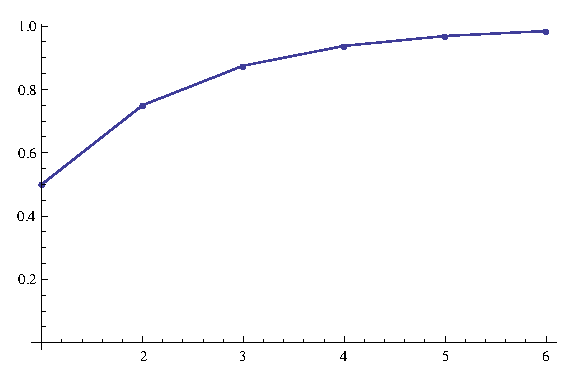
\includegraphics[scale=0.8]{continuous/series/series-3n6n}
        }
        \subfigure[A plot of \( \sum_{n=1}^\infty \frac{2^n}{6^n}. \)]{
          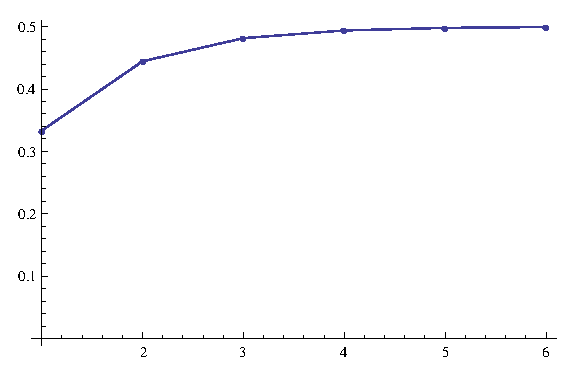
\includegraphics[scale=0.8]{graphs/2pn6pn}
        }
        \subfigure[A plot of \( \sum_{n=1}^\infty \frac{3^n+2^n}{6^n}\).]{
          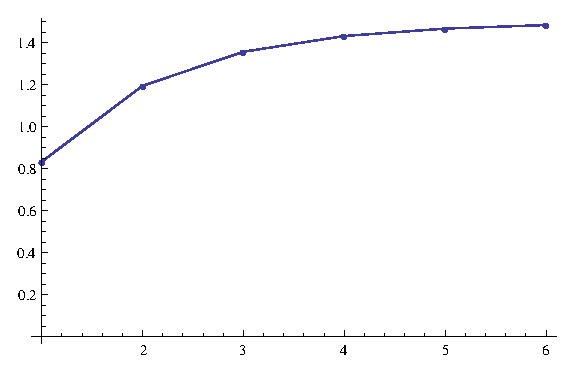
\includegraphics[scale=0.8]{graphs/3pn2pn6pn}
        }
      \end{center}
    \end{figure}

    Finally,
    \begin{align*}
      \sum_{n=1}^{\infty} \frac{3^n+2^n}{6^n}&=\sum_{n=1}^\infty
      \frac{3^n}{6^n} + \sum_{n=1}^\infty
      \frac{2^n}{6^n} \\
      &=1+\frac{1}{2} \\
      &= \frac{3}{2}
    \end{align*}
    The sequence converges to $\frac{3}{2}$.
    \end{sol}
\end{ex}

\section{The Comparison Test}\index{series comparison test}
\begin{theorem}[The Comparison Test]\label{th:seriescomp}
  Let $\sum a_n$, $\sum c_n$, and $\sum d_n$ be series with nonnegative terms.
  Suppose that for some integer $N$
  \[ \forall n > N \bigg(d_n \leq a_n \leq c_n\bigg) \]

  \textbf{(a)} If $\sum c_n$ converges, then $\sum a_n$ also converges.

  \textbf{(b)} If $\sum d_n$ diverges, then $\sum a_n$ also diverges.
\end{theorem}
\cite[p. 559]{thomas}

\section{The Integral Test}\index{series integral test}

Another helpful tool for discovering the behavior of a series is the
\emph{integral test}.
In simple terms, given the following two statements:
\begin{enumerate}
  \item \(f' < 0 \text{ over some interval } [a, \infty) \)
    \item \(f(n)\) is always positive.\footnote{We can often see this by writing out some terms.}
\end{enumerate}
The integral test states that:

\begin{align*}
  \text{\textbf{(a)}} & \sum^\infty_{n=a} f(n) \text{ converges if }
  \int_{a}^{\infty} f(x) \ud x \text{ converges.}  \\
  \text{\textbf{(b)}} & \sum^\infty_{n=a} f(n) \text{ diverges if } \int_{a}^{\infty} f(x) \ud x \text{ diverges.}
\end{align*}

\begin{proof}
  \begin{align*}
    \int^\infty_1 f(x) \ud x
    &\approx f(1) \Delta x + f(2) \Delta x + f(3) \Delta x + \cdots + \text{with } \Delta x = 1 \\
    &\approx f(1) + f(2)+f(3)+\cdots \\
    &\approx \sum^\infty_{n=1} f(n)\qedhere
  \end{align*}
\end{proof}

Here is the official wording for the integral test, copied from \emph{Thomas' Calculus} \cite[p.~554]{thomas}:
\begin{theorem}[The Integral Test]\label{th:seriesint}
  Let $\{a_n\}$ be a sequence of positive terms. Suppose that $a_n = f(n)$,
  where $f$ is a continuous, positive, decreasing function of $x$ for all $x
  \geq N$ ($N \in \mathbb{Z_+}$). Then the series $\sum_{n=N}^\infty a_n$ and
  the integral $\int_N^\infty f(x)\ud x$ both converge or both
  diverge.
\end{theorem}

\begin{ex}\label{famousp}
  Use the integral test to show that the harmonic series diverges.
  \[ \sum^\infty_{n=1} \frac{1}{n} \]
  \begin{sol}
    First, we test it with Theorem \ref{th:nthtermdiv}.
    \[ \lim_{n\to\infty} \frac{1}{n}=0\]
    Because this limit is zero, the test proves inconclusive.

    Let's check the two prerequisites for the integral test. If we let
    $\sum^\infty_{n=1} \frac{1}{n}$ be $\sum^\infty_{n=1}$, and $a_n =
    \frac{1}{n}$, then we can treat $a_n$ as a function and make sure it is
    positive and always decreasing.

    The function \[ f(x)=\frac{1}{x} \]is always positive on $[1, \infty)$.
    Its derivative, \[f'(x)=-\frac{1}{x^2}\] is always negative. Thus, we can
    use the integral test to describe the behavior of $\sum^\infty_{n=1} a_n$.
    \[
      \int^\infty_1 \frac{1}{n} = \lim_{t\to\infty} \ln x \bigg|^\infty_1
    \]
    This integral diverges, so by Theorem \ref{th:seriesint} the series also
    diverges.
%%    Note that it it is better to think:
%%    \[ \sum a_n \to \sum^\infty_{n=\ldots} f(n) \]
%%
%%    \[ \sum^\infty_{n=1} \frac{1}{n} \to \int^\infty_1 \frac{1}{x}\ud x \]
%%    \begin{align*}
%%      \int^\infty_1 \frac{1}{x}\ud x
%%      \text{ is }
%%      \int^t_1 \frac{1}{x} \ud x
%%    \end{align*}
  \end{sol}
\end{ex}
\begin{ex}
  Determine whether the following series is convergent or divergent.
  \[ \sum_{k=4}^\infty k e^{-k^2} \]
  \begin{sol}
    We can use the integral test.
    \begin{align*}
      \int_{k=4}^\infty k e^{-k^2} \ud k
      &=\frac{-1}{2}\int_{k=4}^\infty -2 k e^{-k^2} \ud k \\
      &=\frac{-1}{2}e^{-x^2} \bigg|_4^\infty
    \end{align*}
    \begin{figure}[H]
      \begin{center}
        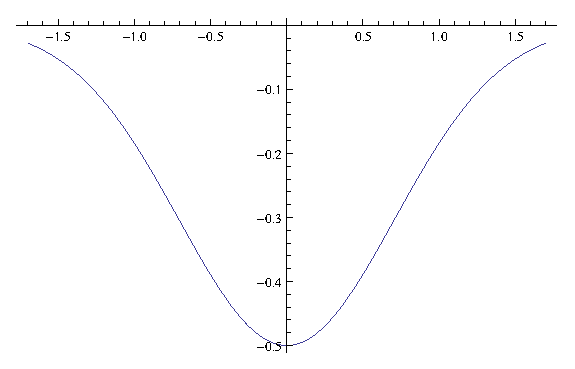
\includegraphics[scale=0.8]{continuous/series/henxs}
      \end{center}
      \caption{A plot of $-\frac{1}{2}e^{-k^2}$}
      \label{fig:henxs}
    \end{figure}
    We can tell that this integral converges, so the series converges.
  \end{sol}
\end{ex}

\section{$p$ Series}
\label{sec:pseries}

A \(p\) series is of the form
\[ \sum_{n=1}^{\infty} \frac{1}{n^p} \]

At \(p=1\), it is a harmonic series and we could say it diverges because of Theorem \ref{th:seriesint}.
Meanwhile, at \(p=2\), the series converges.
If we take \(p=-1\), the series diverges.
At \(p=-2\), the series diverges by Theorem \ref{th:nthtermdiv}.
At \(p=1.0000000000001\), the series converges by the integral test.

We can get a feeling that \( p>1 \) leads to convergence, and \(p \leq 1\) leads to a diverging series.

\section{Series Comparison Test}

\subsection{Converging Series}
\begin{ex}\label{ex:convcomp}
  \[ \sum_{n=1}^{\infty} \frac{5+2\sqrt n}{n^3} \]
  \begin{sol}

    Let $f(x)=\frac{5+2\sqrt{x}}{x^3}$, which is always positive on $x\geq 1$.
    Then $f'(x) = -\frac{5(\sqrt{x}+3)}{x^4}$, which is always negative on $x
    \geq 1$.
    % Something is wrong with these figures.
    % Both have the same caption, yet they are obviously completely different pictures.
    % I should determine how they relate and fix this, or remake them.
    %
    % \begin{figure}[H]
    %   \begin{center}
    %     \subfigure[A plot of $f(x)=\frac{5+2\sqrt{x}}{x^3}$.]{
    %       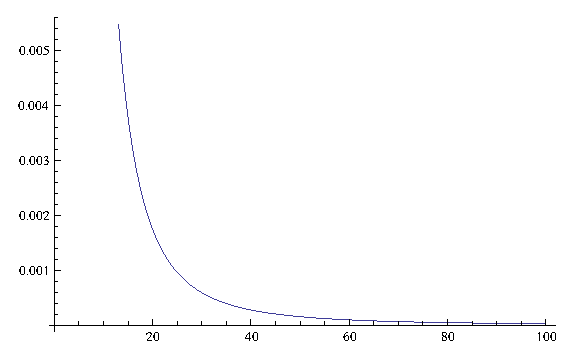
\includegraphics[scale=0.8]{graphs/5p2sqxx3}
    %     }
    %     \subfigure[A plot of $f(x)=\frac{5+2\sqrt{x}}{x^3}$.]{
    %       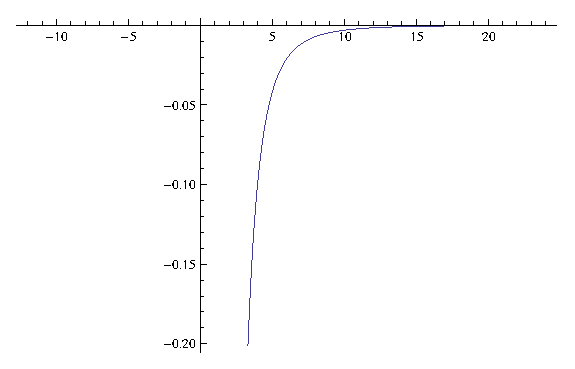
\includegraphics[scale=0.8]{graphs/n5xp3x4}
    %     }
    %   \end{center}
    % \end{figure}
    \begin{align*}
      \int_1^\infty \frac{5+2\sqrt x}{x^3} \ud x
      &= \int_1^\infty \frac{5}{x^3} \ud x
      + \int_1^\infty \frac{2 \sqrt x}{x^3} \ud x \\
      &= \int_1^\infty 5x^{-3} \ud x
      + \int_1^\infty 2x^{1/2} \cdot x^{-3} \ud x \\
      &= \lim_{t\to\infty} \int_1^t 5x^{-3} \ud x
      +  \lim_{t\to\infty}\int_1^t 2x^{-5/2} \ud x \\
      &= \lim_{t\to\infty}\frac{5x^{-2}}{-2}\bigg|_1^t+
      \lim_{t\to\infty}\frac{2x^{-3/2}}{-3/2}\bigg|_1^t \\
      &= \lim_{t\to\infty} \bigg[-\frac{5t^{2}}{2}+\frac{4(1)^{-3/2}}{3} \bigg]
      + \lim_{t\to\infty}\bigg[ -\frac{4t^{-5/2}}{3} +\frac{4(1)^{-3/2}}{3}
        \bigg] \\
      &=\lim_{t\to\infty} \bigg[-\frac{5t^{-2}}{2}+\frac{5}{2} \bigg]
      + \lim_{t\to\infty}\bigg[ -\frac{4t^{-3/2}}{3} +\frac{4}{3}
        \bigg]\\
      &=\lim_{t\to\infty} -\frac{5t^{-2}}{2}+\lim_{t\to\infty} \frac{5}{2}
      + \lim_{t\to\infty} -\frac{4t^{-3/2}}{3} +\lim_{t\to\infty}\frac{4}{3} \\
      &=\frac{23}{6}-\lim_{t\to\infty}\bigg[
        \frac{5t^{-2}}{2}+\frac{4t^{-5/2}}{5} \bigg] \\
      &=\frac{23}{6}-\lim_{t\to\infty}\bigg[
        \frac{5}{2t^2}+\frac{4}{3t^{3/2}} \bigg]\\
        &=\frac{23}{6}+0 \\
        &= \frac{23}{6}
    \end{align*}
    By Theorem \ref{th:seriesint}, the series
    \( \sum_{n=1}^{\infty} \frac{5+2\sqrt n}{n^3} \)
    converges.
  \end{sol}
\end{ex}
\begin{ex}
  \[ \sum_{n=1}^{\infty} \frac{5+2\sqrt{n}}{n^3+1} \]
  We can tell that this is quite similar to Example \ref{ex:convcomp}, except we are making the denominator larger.
  We can tell by comparison with the original problem that this must also converge. Likewise, if we made the numerator smaller, we could treat this as converging.
  For a proper solution, we would write
  \begin{sol}
    \[ \sum_{n=1}^{\infty} \frac{5+2\sqrt{n}}{n^3+1} \]
    Converges by comparison with \( \sum_{n=1}^{\infty} \frac{5+2\sqrt n}{n^3} \).
  \end{sol}
  \begin{figure}[H]
    \begin{center}
      \subfigure[A plot of $s_n=\frac{5+2\sqrt{n}}{n^3}$]{
        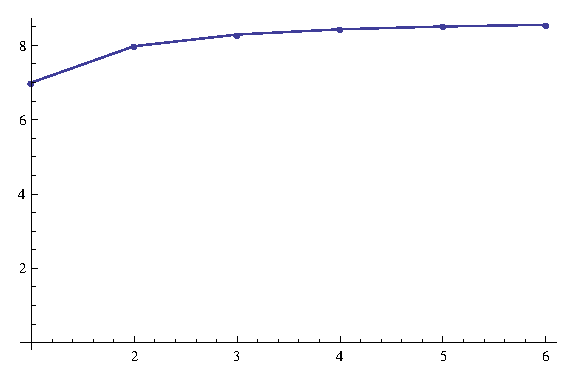
\includegraphics[scale=0.8]{graphs/5p2sqn3}
      }
      \subfigure[A plot of $s_n=\frac{5+2\sqrt{n}}{n^3+1}$]{
        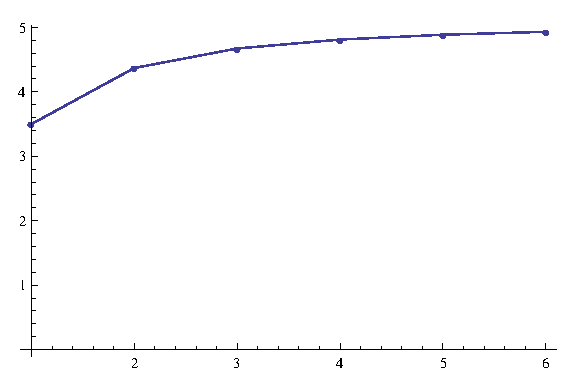
\includegraphics[scale=0.8]{graphs/5p2sqn3p1}
      }
    \end{center}
  \end{figure}

  Make note, however, that making the denominator smaller does not help us in making these comparisons for convergence.
\end{ex}
\begin{ex}
  \[ \sum_{n=1}^{\infty} \frac{1}{n^4} \]
  This is a $p$-series with $p=4$, and therefore converges.

  \[ \sum_{n=1}^{\infty} \frac{1}{n^4+2} \]
  This series converges by comparison with $\sum_{n=1}^\infty \frac{1}{n^4}$.
\end{ex}
\begin{ex}
  \[ \sum_{n=1}^{\infty} \frac{2}{n^2+4n+3} \]
  \begin{note}
    We can use partial fraction decomposition to handle this, and it becomes a telescoping sum.
  \end{note}

  \[ \sum_{n=1}^{\infty} \frac{2}{n^2+4n+6} \]
\end{ex}

\begin{remark}
  Imagine we were dealing with one series that conveges to \( \frac{1}{2} \).
  In turn, we were comparing this with another series that ``shoots off into the negatives.''

  We would have issues comparing these in any way.

  Thus, we must check that \(a_n\) and \(b_n\) are exclusively positive.
\end{remark}

\subsection{Diverging Series}
\begin{ex}
  \[ \sum_{n=1}^{\infty} \frac{n}{n+5} \]
  Using theorem \ref{th:nthtermdiv}, we know that this series diverges.

  \[ \sum_{n=1}^{\infty} \frac{n}{n+5-1} \]

  Here, we are decreasing the size of the denominator for a divergent series.
  We can state that \( \sum_{n=1}^{\infty} \frac{n}{n+5-1} \) diverges by comparison with \( \sum_{n=1}^{\infty} \frac{n}{n+5-1} \).
\end{ex}
\begin{ex}
  \[ \sum_{n=1}^{\infty} \frac{(n+1)^2}{n(n+2)} \]
  Diverges by theorem \ref{th:nthtermdiv}.

  \[ \sum_{n=1}^{\infty} \frac{(n+1)^2}{n(n+2)} \]

  Again, making the denominator smaller. This diverges by comparison with the above series.
\end{ex}
\begin{ex}
  \[ \sum_{n=1}^{\infty} \frac{1}{3n+1} \]
  Diverges.
  \[ \sum_{n=1}^{\infty} \frac{15}{3n+1} \]
  Diverges by comparsion with the above.
\end{ex}
\begin{ex}
  \[ \sum_{n=1}^{\infty} \frac{n+2}{n+1} \]
  Diverges.
  \[ \sum_{n=1}^{\infty} \frac{n(n+2)}{n+1} \]
  It doesn't have to be a constant multiple for the comparison test to work.
  We can still state that this diverges by comparison with the above.
\end{ex}

\section{Root Test}\index{series root test}

\begin{theorem}[Root Test]
  Let \(\sum a_n\) be a series with \( a_n \geq 0\) for \(n \geq N\), and
  suppose that
  \[ \lim_{n \to \infty} \sqrt[n]{a_n} = \rho \]
  then (a) the series \emph{converges} if \(\rho < 1 \), \textbf{(b)} the series
  diverges if \( \rho > 1\) or if \(\rho\) is infinite, or \textbf{(c)} the test
  is \emph{inconclusive} if \(\rho = 1\).
  \cite[p. 565]{thomas}
  \label{th:roottest}
\end{theorem}

\begin{ex}
  Use the root test to determine if the following series converges or diverges.
  \[ \sum_{n=1}^\infty \frac{1}{\left( 5n+7 \right)^n} \]
  \begin{sol}
    The root test tells us that
    \[ \rho = \lim_{n \to \infty} \frac{1}{5n+7} \]
  \end{sol}
\end{ex}
\begin{ex}
  \[ \sum_{n=1}^{\infty} \frac{12}{\left( 3+\frac{1}{n}^{4n} \right)} \]
  \begin{sol}
    Use the root test. Take the \(n\)th root of \(s_n\).
    \begin{align*}
      \rho &= \lim_{n \to \infty} \left[ \frac{12}{ \left( 3+\frac{1}{n}^{4n} \right) }\right]^{1/n} \\
      &= \lim_{n \to \infty} \frac{12^{1/n}}{\left( 3+\frac{1}{n} \right)^4}
      \\
      &= \lim_{n \to \infty} \frac{12^{1/n}}{3^4} \\
      &= \frac{1}{81}
    \end{align*}
  \end{sol}
\end{ex}


\section{Ratio Test}\index{series ratio test}

\begin{theorem}[The Ratio Test]\label{th:seriesratio}
  Let $\sum a_n$ be a series with positive terms and suppose that
  \[ \lim_{n \to \infty} \frac{a_{n+1}}{a_n}=\rho \]
  Then \textbf{(a)} the series \emph{converges} if $\rho < 1$, \textbf{(b)} the
  series \emph{diverges} if $\rho > 1$ or $\rho$ is infinite, \textbf{(c)} the
  test is \emph{inconclusive} if $\rho = 1$.
\end{theorem}

\begin{ex}
  Use the ratio test to determine if the following series converges or diverges.
  \[ \sum^\infty_{n=1} \frac{3^n+n}{n!} \]
  \begin{sol}
    First, let's look at the series:
    \[ \frac{4}{1} + \frac{11}{3} + \frac{30}{6} + \cdots \]

    Just use the ratio test, which we can do because this series has exclusively
    positive terms.
    \begin{align*}
      \lim_{n \to \infty}
      \cfrac{\cfrac{3^{n+1}+(n+1)}{(n+1)!}}{\cfrac{3^n+n}{n!}}
      &= \lim_{n \to \infty} \cfrac{(n!)\bigg(3^{n+1}+(n+1)\bigg)}{(3^n+n)(n+1)!} \\
      \intertext{It is important to note here that by factoring a $n+1$ term out
        of $(n+1)!$, we find that $(n+1)! = (n+1)n!$. This
      allows us to manipulate our limit so that some terms will cancel.}
      &= \lim_{n \to \infty}
      \cfrac{(n!)\bigg(3^{n+1}+n+1\bigg)}{(3^n+n)(n+1)(n!)} \\
      &= \lim_{n\to\infty} \frac{3^{n+1}+n+1}{(3^n+n)(n+1)} \\
      &= \lim_{n\to\infty} \frac{3^{n+1}+n+1}{n3^n+n^2+3^n+n} \\
      &= \lim_{n\to\infty}
      \cfrac{\cfrac{3^{n+1}}{3^{n+1}}+\cfrac{n}{3^{n+1}}+\cfrac{1}{3^{n+1}}}
      {\cfrac{n(3^n)}{3^{n+1}}+\cfrac{n^2}{3^{n+1}}+\cfrac{3^n}{3^{n+1}}+\cfrac{n}{3^{n+1}}}
      \intertext{
        Now, as \(n \to \infty\) many of the terms disappear. $n3^n/3^{n+1}$
      becomes $n/3$.}
      &= \lim_{n\to\infty} \cfrac{1}{\frac{n}{3}+\cfrac{1}{3}}\\
      &=\lim_{n \to \infty} \frac{3}{n+1}\\
      &=0
      % &= \lim_{n \to \infty} \frac{3^{n+1}+n+1}{(n+1)(3^n+n)}\\
      % &= \lim_{n \to \infty} \frac{3^{n+1}+n+1}{n3^n+n^2+3^n+n} \\
      % &= \lim_{n \to \infty} \cfrac{3^n \left(
      %  3+\cfrac{n}{3^n}+\cfrac{1}{3^n} \right)}{3^n\left(
      %  n+\cfrac{n^2}{3^n}+1+\cfrac{n}{3^n} \right)} \\
      % &= \lim_{n \to \infty} \cfrac{3+\cfrac{n}{3^n}+\cfrac{1}{3^n}}{n+
      %   \cfrac{n^2}{3^n}+1+\cfrac{n}{3^n}}
    \end{align*}
    Thus, by \ref{th:seriesratio}, this series converges.
    \begin{remark}
      \begin{align*}
        \lim n \to \infty \frac{n}{3^n} \=H \frac{1}{\ln 3 e^{n \ln 3}}
    \end{align*}
    \end{remark}
  \end{sol}
\end{ex}
\begin{ex}
  Use the ratio test to determine if the following series converges or diverges.
  \[ \sum_{n=1}^\infty \frac{n^{19}}{19^n} \]
  \begin{sol}
    Use the ratio test.
    \begin{align*}
      \lim_{n \to \infty}
      \cfrac{\cfrac{(n+1)^{19}}{19^{n+1}}}{\cfrac{n^{19}}{19^n}}
      &= \lim_{n \to \infty} \cfrac{19^n \cdot (n+1)^{19}}{19^{n+1}\cdot n^{19}} \\
      \intertext{$19^n / 19^{n+1}$ becomes just $19$.}
      &= \lim_{n \to \infty} \cfrac{(n+1)^{19}}{19 \cdot n^{19}}
      \intertext{Note that there's no way the \((n+1)^{19}\) and \(n^19\) can in
      any way cancel. However, were we to foil the \((n+1)^{19}\) nineteen
      times, the leading term would be \(n^{19}\). The limit is, therefore, just
    the limit}
    &= \lim_{n \to \infty} \frac{n^{19}}{19n^{19}} \\
    &= \frac{1}{19}
    \end{align*}
  \end{sol}
\end{ex}

\subsection{Examples}

\begin{ex}
  Does
  \[ \sum_{n=1}^{\infty} \frac{1}{2^n} \]
  converge or diverge?
  \begin{sol}
    \begin{align*}
      s_1 &= \frac{1}{2} \\
      s_2 &= \frac{1}{2} + \frac{1}{4} \\
      s_3 &= \frac{1}{2}+ \frac{1}{4} + \frac{1}{8} \\
      s_4 &= \frac{1}{2}+ \frac{1}{4} + \frac{1}{8} + \frac{1}{16} \\
      s_n &= \frac{2^n-1}{2^n}
    \end{align*}
  \end{sol}
\end{ex}
\begin{ex}
  Does
  \[\sum_{n=2}^{\infty} \frac{n+10}{10n+1} \]
  converge or diverge?
  \begin{align*}
    \lim_{n \to \infty} \frac{n+10}{10n+1} = \\
    \intertext{Divide all terms by \(n\).}
    & \frac{\frac{n}{n}}{\frac{10n}{n}}&=\frac{1}{10} \neq 0 \\
  \end{align*}
  Therefore, the series diverges.
\end{ex}
\begin{ex}
  \[ \sum_{n=0}^\infty \frac{4}{2^n} \]
  \begin{sol}
    Theorem \ref{th:nthtermdiv} gets us nowhere with this one. In other words,
    \[ \lim_{n \to \infty} \frac{4}{2^n} = 0 \]
    is inconclusive.

    We have a geometric series.
    \[ 4 \left( 1+ \frac{1}{2} + \frac{1}{4} + \frac{1}{8} + \frac{1}{16} + \cdots \right) = \frac{1}{1-\frac{1}{2}} \]
    So
    \[ \sum{n=0}^\infty \frac{4}{2^n} \]
    converges to \(8\).
  \end{sol}
\end{ex}
\begin{ex}
  Does
  \[ \sum_{n=1}^\infty \frac{1}{n}-\frac{1}{n-2} \]
  converge or diverge?
  \begin{sol}
    Check the limit.
    \begin{align*}
      \lim_{n \to \infty} \frac{1}{n} - \frac{1}{n-2} &=
      \lim_{n \to \infty} \frac{n-2}{n(n-2)} - \frac{n}{n(n-2)} \\
    \end{align*}
    \[
      \frac{1}{1}-\frac{1}{3}+\frac{1}{2}-\frac{1}{4}+\frac{1}{3}-\frac{1}{5}+\cdots
    \]
    This is called a telescoping sum that converges to \(\frac{3}{2}\).
  \end{sol}
\end{ex}
\begin{ex}
  \[ \sum_{n=1}^{\infty} \frac{n+1}{2n-1} \]
  \begin{sol}
    Check the limit.
    \[ \lim_{n \to \infty} \frac{n+1}{2n-1}\neq0 \]
    The series diverges.
  \end{sol}
\end{ex}
\begin{ex}
  \[ \sum_{n=1}^{\infty} \frac{3n-1}{2n+1} \]
  Check the limit.
    \[ \lim_{n \to \infty}\frac{3n-1}{2n+1}\neq0 \]
    The series diverges.
\end{ex}
\begin{ex}
  \[ \sum_{n=0}^{\infty} \frac{1}{4^n} \]
  \begin{sol}
    \[ \frac{1}{1}+\frac{1}{4}+\frac{1}{16}+\frac{1}{32}+\ldots \]
    Converges to \(\frac{1}{1-\frac{1}{4}}\).
  \end{sol}
\end{ex}
\begin{ex}
  \[ \sum_{n=0}^{\infty} (1.075)^n \]
  \begin{sol}
    $\lim_{n\to\infty} (1.075)^n\neq0$ and the series diverges because of
    Theorem \ref{th:nthtermdiv}.
  \end{sol}
\end{ex}
\begin{ex}
  \[ \sum_{n=1}^\infty \frac{2^n}{100} \]
  \begin{sol}
    $\lim_{n\to\infty} \frac{2^n}{100}\neq 0$ so by Theorem \ref{th:nthtermdiv}
    the series diverges.
  \end{sol}
\end{ex}
\begin{ex}
  \[ \sum_{n=1}^\infty \frac{2^n}{n^2} \]
  \begin{sol}
    \(2^n\) is geometric but the \(n^2\) denominator means we can't treat it
    like a geometric series.

    Using Theorem \ref{th:nthtermdiv}, we find that
    \begin{align*}
      \lim_{n\to\infty} \frac{2^n}{n^2}&=\lim_{n\to\infty} \frac{e^{n\ln2}}{n^2}
      \\
      &\=H \lim_{n\to\infty} \frac{\ln 2 e^{n \ln 2}}{2n} \\
      &\=H \lim_{n\to\infty} \frac{2\ln 2 e^{n \ln 2}}{2} \\
      &\neq 0
    \end{align*}
    so the series diverges.
  \end{sol}
\end{ex}
\begin{ex}
  \[ \sum_{n=1}^\infty \frac{1}{n(n+3)} \]
  \begin{sol}
    Checking with \ref{th:nthtermdiv} proves inconclusive.

    We can use partial fraction decomposition on this fraction.
    \begin{align*}
      \frac{1}{n(n+3)} =& \frac{A}{x}+\frac{B}{x+3} \\
      \intertext{We find that \( A = \frac{1}{3} \) and \(B = -\frac{1}{3} \)}
      =& \frac{1/3}{x}-\frac{1/3}{x+3}
    \end{align*}

    \begin{align*}
      \sum_{n=1}^\infty \frac{1}{n(n+3)} =& \frac{1}{3} \sum_{n=1}^\infty \left(\frac{1}{n}-\frac{1}{n+3}\right)
    \end{align*}
  \end{sol}
\end{ex}
\begin{ex}
  \[ \sum^\infty_{n=4} \frac{1}{(n-3)^2} \]
  \begin{sol}
    Check it with Theorem \ref{th:nthtermdiv}:
    \[ \lim_{n \to \infty} \frac{1}{(n-3)^2} = 0 \]
    Which is inconclusive, so we will attempt to use the integral test.
    \[ f(x) = \frac{1}{(x-3)^2} \]
    Check the derivative:
    \begin{align*}
      f'(x) &= \frac{(x-3)^2 \frac{\ud}{\ud x}(1) - 1 \frac{\ud}{\ud x}(x-3)^2} {(x-3)^4} \\
        &= \frac{-2(x-3)}{(x-3)^4} \\
        &= \underbrace{\frac{-2}{(x-3)^3}}_{\text{DNE when } x=3 }
    \end{align*}
    \begin{table}[h]
      \centering
      \boxed{
        \begin{tabular}{r|c|c|c}
          $x$ & $-\infty$ & $3$ & $\infty$ \\ \hline
          $f(x)$ & \multicolumn{3}{c}{$+$} \\ \hline
          $f'(x)$ & $-$ & \text{ undefined } & $-$
        \end{tabular}
      }
      \caption{A sign diagram of $f(x)$ and $f'(x)$}
    \end{table}
    $f(x)$ is always positive, and $f'(x)$ is always negative, so the first two prerequisites for theorem \ref{th:seriesint} are passed.

    Now consider
      \[ \int^\infty_4 \frac{1}{(x-3)^2} \ud x  \]
    {First evaluate this as an indefinite integral:}
    \begin{align*}
      \int \frac{1}{(x-3)^2}\ud x
      &=\int \frac{1}{u^2}\ud u =\int u^{-2} \ud u \\
      &=\frac{u^{-1}}{-1} \\
      &=\frac{-1}{(x-1)}
    \end{align*}
      {Now evaluate it in terms of the original definite integral:}
    \begin{align*}
      \int^\infty_4 \frac{1}{(x-3)^2} \ud x
      &=\lim_{t\to\infty} \frac{-1}{(x-1)}\bigg|^t_4 \\
      &=-\lim_{t\to\infty} \frac{1}{(t-1)}+\frac{1}{3} \\
      &=-\frac{1}{3}
    \end{align*}
    This integral converges, so the $\sum^\infty_{n=4}
    \frac{1}{(n-3)^2}$ must converge (though we don't know to what).
  \end{sol}
\end{ex}
\begin{homework}
  \date{30 March 2012}

  Read Section 10.4

  pg. 562 \# 1, 3, 5, 6 (converges by comparison with \(\frac{1}{3^n}\), 7, 33, 35, 37, 41, 47
\end{homework}
\begin{ex}
  Does the following series converge or diverge?
  \[ \sum_{n=1}^\infty \frac{\ln n}{n} \]
  \begin{sol}
    Check Theorem \ref{th:nthtermdiv} first and foremost.
    \begin{align*}
      \lim_{n \to \infty} \frac{\ln n}{n}
      &\=H \lim_{n \to \infty} \frac{\frac{1}{n}}{1} \\
      &= 0
    \end{align*}

    Next, check with the integral test, theorem \ref{th:seriesint}.

    We know that the \(\ln x\) is positive past \(x=1\), so the second condition
    for use of the theorem is satisfied.

    The first condition is slightly more difficult:

    \begin{align*}
      f' &= \frac{x \cdot \frac{1}{x}- \ln x}{x^2} \\
      &= \frac{1- \ln x}{x^2}
    \end{align*}

    Which is \( > 0 \), so we can use the integral test.

    \begin{align*}
      \int_{1}^{\infty} \frac{\ln n}{n} \ud x \\
      \frac{(\ln x)^2}{2} \bigg|_{1}^{\infty}
    \end{align*}

    We can conclude that the series diverges.
  \end{sol}
\end{ex}
\begin{ex}
  Does the following series converge or diverge?
  \[ \sum^\infty_{n=1} \frac{3}{\sqrt{n}} \]
  \begin{sol}
    Recognize this as a \(p\)-series with \(p=1/2\).

    Note that, without the \(3\), we would be looking at a definitely diverging
    \(p\)-series.

    However, multiply that diverging series by \(3\) and we are dealing with an
    even \emph{bigger} diverging \(p\)-series.

    The series, therefore, diverges by comparison with \[
      \sum_{n=1}^\infty \frac{1}{\sqrt{n}} \]
  \end{sol}
\end{ex}
\begin{ex}
  Determine if this geometric series converges or diverges. If it converges,
  find its sum.
  \[ (1/5) + (1/5)^2 + (1/5)^3 + (1/5)^4 + \cdots \]
  \begin{sol}
    Treat it as a geometric series and multiply it as such.
    \[ \left( 1-\frac{1}{5} \right) \left(\frac{1}{5} + (1/5)^2 + (1/5)^3 + (1/5)^4 +
      \cdots \right) = \frac{1}{5} \]
    So now we look for our final answer:
    \begin{align*}
      \frac{\frac{1}{5}}{1-\frac{1}{5}} = \frac{1}{4}
    \end{align*}
  \end{sol}
\end{ex}
\begin{ex}
  If the series \[ \sum^{\infty}_{n=0} \cos{9n\pi} \] converges, then what is
  its sum.
  \begin{sol}
    This turns out to just be a fancy way of writing
    \[ \sum 1-1+1-1+1-1+1-1+\cdots \]

    Alternatively, we are talking about a cosine function. The cosine function
    never settles down, it constantly jumps back and forth between values. Thus,
    we could take the limit as \( n \to \infty\) of \(s_n\) to find that it
    diverges.
  \end{sol}
\end{ex}
\begin{ex}
  Find a formula for the \(n\)th partial sum of the series and use it to
  determine if the series converges.
  \[ \sum_{n=1}^\infty (\ln \sqrt{n+1} - \ln \sqrt{n}) \]
  \begin{sol}
    \begin{align*}
      s_1 &= \ln \sqrt{2} - \ln \sqrt 1 \\
      s_2 &= \ln \sqrt 3 - \ln \sqrt 2 + \ln \sqrt 2 - \ln \sqrt 1 \\
      s_3 &= \ln \sqrt 4 - \ln \sqrt 3 + \ln \sqrt 3 + \ln \sqrt 2 - \ln \sqrt 1
      \\
      s_4 &= \ln \sqrt 5 - \ln \sqrt 4 + \ln \sqrt 4 - \ln \sqrt 3 + \ln \sqrt 3
      - \ln \sqrt 2 + \ln \sqrt 2 - \ln \sqrt 1 \\
      s_5 &= \ln \sqrt 6 - \ln \sqrt 5 + s_4 \\
      s_n &= \ln \sqrt{n+1}-\ln \sqrt{1}
    \end{align*}
    \[ \sum^\infty_{n=1} \text{ is } s_\infty \]
    We can conclude that the series diverges.
  \end{sol}
\end{ex}
\begin{ex}
  Use the limit comparison test to determine convergence or divergence.
  \[ \sum^\infty_{n=1} \frac{n}{n^2 + 7n +5} \]
  \begin{sol}
    \begin{align*}
      \lim_{n \to \infty} \frac{\frac{n}{n^2+7n+5}}{\frac{1}{n}} =1
    \end{align*}
    This is about the same order of magnitude as our original problem. The
    numerator and the denominator balance, and the limit takes us to 1, so the
    series diverges.
  \end{sol}
\end{ex}
\begin{ex}
  Tell whether the series converges or diverges. If it converges, give its sum.
  \[ 1 + \frac{8}{9} + \left( \frac{8}{9} \right)^2 + \left(
    \frac{8}{9} \right)^3+ \cdots + \left( \frac{8}{9} \right)^n + \cdots \]
  \begin{sol}
    Treat this as a geometric series.

    We will find the answer converges to $9$.
  \end{sol}
\end{ex}
\begin{ex}
  Does the series
  \[ \sum^\infty_{n=1} \frac{5}{n^2+36} \]
  converge or diverge? If so, to what?
\end{ex}
\begin{ex}
  If the series \[ \sum_{n=0}^\infty \left( \frac{3}{\sqrt{13}} \right)^n \]
  converges, what is its sum?
  \begin{sol}
    \[\left( 1-\frac{3}{\sqrt{13}} \right) \left[ 1+\frac{3}{\sqrt{13}}+\left( \frac{3}{\sqrt{13}} \right)^2+\ldots \right] \]
  \end{sol}
\end{ex}
\begin{ex}
  Find a formula for the \(n\)th partial sum of the series.
  \[ \sum^\infty_{n=1} \left( \frac{1}{n}-\frac{1}{n+1} \right) \]
  \begin{sol}
    \[ s_n = 1-\frac{1}{n+1} \]
  \end{sol}
\end{ex}
\begin{ex}
  Does the series
  \[ \sum^\infty_{n=1} \frac{4e^n}{1+e^{2n}} \]
  converge or diverge?
  \begin{sol}
    This series is a variation of
    \begin{align*}
      \sum^\infty_{n=1} \frac{4e^n}{e^{2n}} &=
      4 \sum^\infty_{n=1} \frac{e^n}{e^{2n}} \\
      &= 4 \sum^\infty_{n=1} \left( \frac{1}{e} \right)^n
    \end{align*}
    Which is a geometric series.

    The original series converges by comparison with the above.
  \end{sol}
\end{ex}
\begin{ex}
  Use the limit comparison test to determine if the following series converges
  or diverges by comparison with \(\sum^\infty_{n=2} \frac{1}{n} \).
  \[ \sum^\infty_{n=2} \frac{1}{\ln n} \]
  \begin{sol}
    Remember that the limit comparison test is far different from the comparison
    test.
    \begin{align*}
      \lim_{n \to \infty} \frac{\frac{1}{\ln n}}{\frac{1}{n}} &=
      \lim_{n \to \infty} \frac{n}{\ln n} \\
      \=H \lim_{n \to \infty} \frac{1}{\frac{1}{n}} \\
      &= \lim_{n \to \infty} n
    \end{align*}
    \(n\) diverges as it goes toward \(\infty\).
  \end{sol}
\end{ex}

\section{Alternating Series Test}

\begin{theorem}[Leibniz's Test]\index{Leibniz's Test}\index{alternating series
  test}\label{th:alternatingseries}\cite[p.~568]{thomas}
  The series
  \[ \sum^\infty_{n=1} (-1)^{n+1} u_n = u_1 - u_2 + u_3 - u_4 + \cdots \]
  converges if all three of the following conditions are satisfied:
  \begin{enumerate}
    \item The $u_n$'s are all positive.
    \item The postive $u_n$'s are (eventually) noincreasing: $u_n \leq u_{n+1}
      for all n \geq N$, for some integer $N$.
    \item $u_n \to 0$
  \end{enumerate}
  \begin{note}
    Also known as the alternating series test.
  \end{note}
\end{theorem}
\begin{proof}
  Let's write out some of the terms of an alternating series, see how it's
  playing out:
  \[ u_1 - u_2 + u_3 - u_4 + \cdots\]
  \begin{remark}
    These could start negative, too, and we would just factor that out of the sum
    to make it postive and fit the theorem.
  \end{remark}
  \begin{align*}
    s_2 &= u_1 - u_2 \geq 0 \\
    s_4 &= s_2 + (u_3 - u_4) \geq s_2 \\
    s_6 &= s_4 + (u_5 - u_6) \geq s_4
  \end{align*}
  So we see, at each step, that the sequence of partial sums is monotonic
  increasing. To know that it converges, we mus first show that it is bounded.

  The sequence of partial sums gets larger and larger so the lower bound is
  \[ s_n = u_1 - \overbrace{(u_2 - u_3)}^+ - \overbrace{(u_4 - u_5)}^+ \]
  The \emph{sequence of partial sums} is monotonic and bounded by $M=u$ and
  $m=s_2$.

  Therefore, the series converges.
\end{proof}
\begin{ex}
  \[ \sum^\infty_{n=1} (-1)^n \frac{3n}{4n-1} \]

  Although at first this appers to be an alternating series, it actually
  diverges by Theorem \ref{th:nthtermdiv}, the limit test.
\end{ex}
\begin{ex}
  \[ \sum^\infty_{n=1} (-1)^{n+1} \left( \frac{3n+2}{4n^2+3} \right) \]
  \begin{sol}
    Check with \ref{th:nthtermdiv}, which proves inconclusive.

    Take the derivative of $f(x)=(-1)^n \frac{3n}{4n-1}$. We find $f'(x)$ is
    negative everywhere.
    \begin{align*}
      f'(x)&=12x^2-9-24x^2-16x \\
      f'(x)&=-12x^2-16x-9
    \end{align*}
    By Theorem \ref{th:alternatingseries}, this series converges.
  \end{sol}
\end{ex}

So far, we've been able to tell to what number very few infinite sums converge.
Geometric and telescoping sums, for example. For convergent alternating series,
we can always estimate the limit, $L$, and measure the error of our estimation,
the discrepancy between this estimate and the actual theoretical value of
$L$.\footnote{There's an awesome diagram about this in the textbook. Check out
  \cite[p.~569 Fig.~10.13]{thomas}.}

This error is given by
\begin{equation}
  \pm | L - S_n |
\end{equation}

\begin{homework}
  Read section 10.8

  pg 588 odd 1-9, 11, 13, 23, 25, 27
\end{homework}

\section{Power Series}\index{Power Series}[Thomas' Calculus pg 575]
A \textbf{power series} about $x=0$ is the form
\[ \sum_{n=0}^\infty c_n x^n = c_0 + c_1 x + c_2 x + \cdots. + c_n x^n + \cdots
  \]
  And a power series about $x=a$ is of the form
  \begin{equation}\label{eq:powerxa} \sum_{n=0}^\infty c_n (x-a)^n = c_0 + c_1 (x-a) + c_2 (x-a)^2 +
    \cdots + c_n (x-a)^n + \cdots \end{equation}
    in which the center $a$ and the coefficicents $c_0, c1, c2, \cdots$ are
    constants.

    Taking all the coefficients to be $1$ in equation \eqref{eq:powerxa}
    gives us the \textbf{geometric series}\index{geometric series}
    \begin{equation}\label{eq:geopower}
      \szinfty x^n = 1 + x + x^2 + x^3 + x^4 + x^5 + \cdots + x^n  + \cdots
    \end{equation}
    \begin{figure}[H]
      \begin{center}
        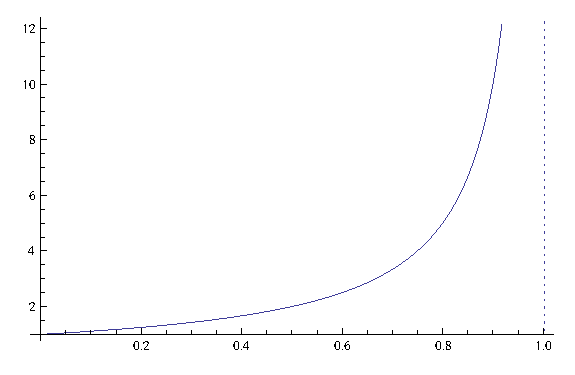
\includegraphics{continuous/series/geopower}
      \end{center}
      \caption{A plot of equation \eqref{eq:geopower}.\label{fig:geopower}}
    \end{figure}
    This is the geometric series with the first term $1$ and the ratio $x$.
    It converges to $1/(1-x)$ for $|x|<1.$ As shown in Figure
    \ref{fig:geopower}, the series has a vertical asymtote at $x=1$ and we
    cannot approximate it at $x \geq 1$.
    \begin{theorem}
      [Reciprocal Power Series]\index{reciprocal power
      series}\label{th:recipowser}
      \begin{equation}
        \frac{1}{1-x} = \sum_{n=0}^{\infty}x^n, \quad |x| < 1
      \end{equation}
    \end{theorem}
\begin{ex}
  \[ \sum^\infty_{n=0} n^3 x^n   \]
  An example of a \textbf{power series}, where the coefficient depends on where
  you are adding the polynomial.\label{powerseriesex1}
  Otherwise described as a \emph{power series about \(x=0\)}.
\end{ex}
\begin{ex}
  \[\sum^\infty_{n=0} n^3 (x-5)^n\]
  This is nothing more than example \ref{powerseriesex1} shifted 5 to the right.
  Otherwise described as a \emph{power series about \(x=5\)}.
  \begin{sol}
    Ratio test.
    \begin{align*}
      \lim{n\to\infty} \bigg| \frac{(n+1)^3 (x-5^{n+1}}{n^3 (x-5)^n} \bigg|
      &=
      \lim{n\to\infty} \bigg| \frac{(n+1)^3 (x-5^{1}}{n^3} \bigg| \\
      \intertext{Factor out the polynomial and take the limit by dividing each
      term by the highest power.}
      &= | x-5| \cdot \lim_{n\to \infty} \frac{n^3+3n^2+3n+1}{n^3} \\
      &= |x-5| \cdot 1 \\
      &= |x-5|
    \end{align*}
    \[ |x-5| < 1 \]
    This has an interval of convergence from $4$ to $6$.
    \begin{note}
      For this to be correct, we \textbf{must} consider:
      \[ \sum^\infty_{n=0} n^3 (6-5)^n \]
      This one diverges by the \emph{nth term test}.
      \[ \sum^\infty_{n=0} n^3 (4-5)^n \]
      because the ratio test is inconclusive at $x=1$.
      Although this is an alternating series, this one diverges by the \emph{nth
      term test}.

      The interval $(4, 6)$ is the interval of convergence. This interval is
      \emph{about} $x \approx 5$.

      This is sometimes called a ``radius of convergence\index{radius of
      convergence},'' drawn as a circle on
      a number line.
    \end{note}
  \end{sol}
\end{ex}
We want to talk about what kind of $x$ values will result in a finite sum, or
infinite sum.
\begin{note}
  An interval of convergence can be $-\infty<x<\infty$. The radius of
  convergence would thus be $\infty$.
\end{note}
\begin{ex}
  An interval of convergence from $3 < x < 7$. The radius of convergence is $2$.
\end{ex}

\section{Taylor and Maclauren Series}

A \textbf{Taylor Series}\index{Taylor series} is an approximation of a function using a power series.

  We do so by treating this function as the sum of a power series
  \begin{align*}
    f(x) &= \sum^\infty_{n=1} a_n(x-a)^n \\
    f(x) &= a_0+a_1(x-a)+a_2 (x-a)^2 + a_3 (x-a)^3 + \cdots a_n (x-a)^n + \cdots
  \end{align*}
  If we differentiate this power series, we get
  \begin{align*}
    f(x) &= a_0+a_1(x-a)+a_2 (x-a)^2 + a_3 (x-a)^3 + \cdots a_n (x-a)^n + \cdots \\
    f'(x) &= 0+a_1+2a_2 (x-a) +3 a_3 (x-a)^2 + \cdots n a_n (x-a)^{n-1} + \cdots \\
    \intertext{Differentiate it again, and we get}
    f''(x) &= 1 \cdot 2a_2+2 \cdot 3 a_3 (x-a) + 3 \cdot 4 a_4 (x-a)^2 + \cdots + (n-1)n a_n (x-a)^{n-2} + \cdots \\
    \intertext{Further differentiation leaves us}
    f'''(x) &= 2 \cdot 3 a_3 + 2 \cdot 3 \cdot 4 a_4 (x-a) + 3 \cdot 4 \cdot 5 a_5 (x-a)^2 + \cdots
  \end{align*}
  So the $n^\textrm{th}$ derivative, for all $n$, is
  \[ f^n(x) = n! a_n + \textrm{a sum of terms with $(x-a)$ as a factor.} \]
  All these equations are perfect approximations of $f(x)$ at $x=a$, though repeated differentiation makes them more accurate as we get further from that value.
  This property allows us to state that $f'(a)=a_1$, $f''(a)=1 \cdot 2 a_2$, $f'''(a)=1 \cdot 2 \cdot 3 a_3$, and
  \[ f^{(n)}(a) = n! a_n.\]
  This shows us that, if $f(x)$ \emph{has} a power series representation, then its $n^\textrm{th}$ term coefficient is
  \[ a_n = \frac{f^{(n)}(a)}{n!}. \]
  \cite[p. 584]{thomas}

  \begin{theorem}[Taylor's Theorem]
    Let $f$ be a function with derivatives of order $k$ for $k=1, 2, \cdots, N$ in some interval containing $a$ as in interior point.
    Then $\forall (n\in \mathbb{Z})$ from $0$ through $N$, the Taylor polynomial of order $n$ generated by $f$ at $x=a$ is the polynomial
    \begin{equation}
      P_n(x)=f(a)+f'(a)(x-a)+\frac{f''(a)}{2!}(x-a)^2+\cdots+\frac{f^{(k)}(a)}{k!}(x-a)^k+\cdots+\frac{f^{(n)}(a)}{n!}(x-a)^n
    \end{equation}
    \cite[p. 586]{thomas}
    \label{th:taylor}
  \end{theorem}

We don't normally treat these as infinite series, as that defeats the purpose of using a series produce a simplified version of a function.

\begin{theorem}
  The Taylor series of a function around a point $x=a$ is
  \[ f(x) \approx f(a) + \frac{f'(a)}{1!}(x-a) + \frac{f''(a)}{2!}(x-a)^2+\frac{f^{(3)}(a)}{3!}(x-a)^3+\cdots . \]
  \label{th:taylorseries}
\end{theorem}
If this Taylor Series is calculated about $x=0$, we call it a \textbf{Maclauren Series}\index{Maclauren Series}.
\begin{ex}
   Say we are trying to approximate the function
  \[ f(x) =  e^x \]
  around $x=1$.
  \begin{figure}[H]
    \begin{center}
      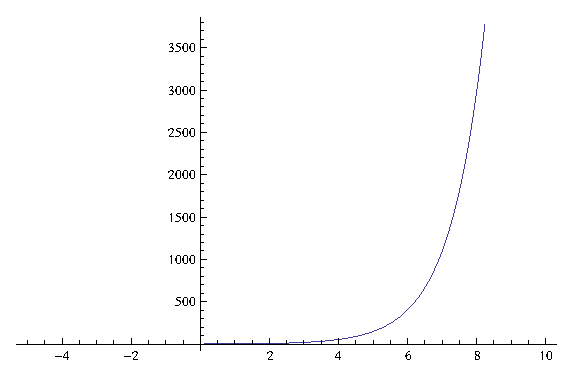
\includegraphics{continuous/series/etx}
    \end{center}
    \caption{A plot of $f(x)=e^x$.}
  \end{figure}
  For the simplext possible approximation, we would just calculate the function at $x=1$ and that would be our solution.
  This is a constant function and is called a \textbf{0$^\textrm{th}$ order approximation}.
  \[f(x) \approx e \]
  To improve our approximation, we increase the power of our Taylor series.
  \begin{align*}
    f(x) &\approx a_0 + a_1 (x-a)\\
    f(x) &\approx e + e (x-1)
  \end{align*}
  \begin{figure}[H]
    \begin{center}
      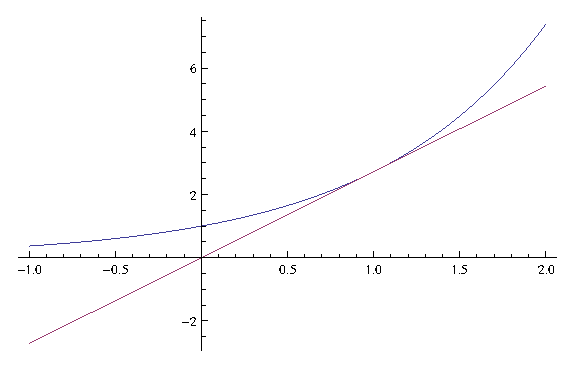
\includegraphics{continuous/series/1storder}
    \end{center}
    \caption{A plot of $e^x$ and $e+e(x-1)$.}
  \end{figure}
  We can improve it even further by increasing our number of terms:
  \begin{align*}
    f(x) &\approx a_0 + a_1 (x-a) + a_2 (x-a)^2 \\
    \intertext{We already know the first two coefficients, so}
    f(x) &\approx e + e (x-a) + a_2 (x-a)^2 \\
    \intertext{To find $a_2$, we take the second derivative of $f(x)$ at $x=1$ and divide that by $2!$.}
    f(x) &\approx e + e (x-a) + \frac{e}{2!} (x-a)^2 \\
  \end{align*}
  \begin{figure}[H]
    \begin{center}
      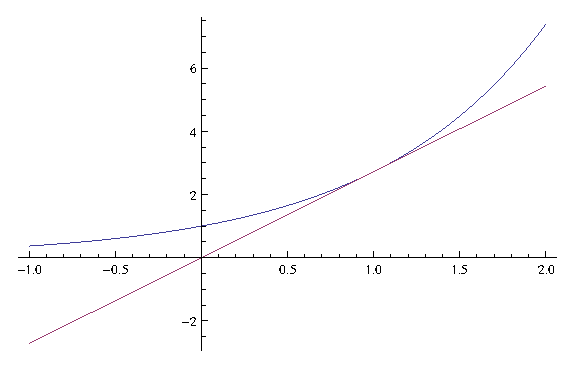
\includegraphics{continuous/series/1storder}
    \end{center}
    \caption{A plot of $e^x$ and $e+e(x-1)+\frac{e}{2!} (x-a)^2$.}
  \end{figure}
\end{ex}
\begin{comment}
  \begin{ex}
    Say we are trying to approximate the function
    \[ f(x) =  e^x \]
    \begin{figure}[H]
      \begin{center}
        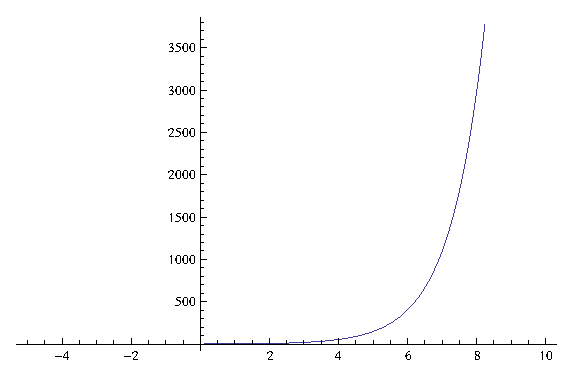
\includegraphics{continuous/series/etx}
      \end{center}
      \caption{A plot of $f(x)=e^x$.}
      \label{fig:etx}
    \end{figure}
    Before we start, we must decide \emph{where} we are going to make the
    approximation.
    Say we are approximating this function around $x=1$.

    For the simplext possible approximation, we would just calculate the function at $x=1$ and that would be our solution.
    \begin{align*}
      f(x) &\approx f(a) \\
      f(x) &\approx e
    \end{align*}
    This is a constant function and is called a \textbf{0$^\textrm{th}$ order approximation}.
    \begin{figure}[H]
      \begin{center}
        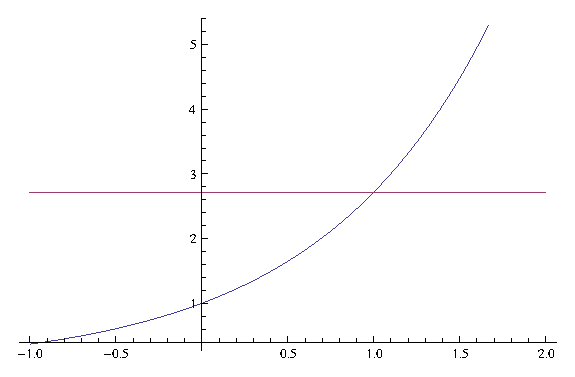
\includegraphics{continuous/series/etx2}
      \end{center}
      \caption{A plot of $e^x$ and $e$.}
      \label{fig:etx2}
    \end{figure}
    This can get the slope right at one point.
    But, if we want to create a more accurate approximation, we would need to include the derivative of the function around $x=1$.

    Treat this function as a y value. The $y$ values is $e^1$.
    \[e^1=c_0+c_1 (x-a)\]
    We have one equation and two unknowns. We should also, here, approximate the
    slope of $e^x$ at $x=1$.
    \begin{align*}
      f'(x)&=c_0+c_1 \cdot 1 \\
      \ddx e^x \bigg|_{x=1} &\equiv c_1
    \end{align*}
    To solve this, recognize $c_1$ is $e^1$. Plug this into the first equation for
    your coefficients.

    \[ f(x) = c_0 + c_1x + c_2x^2 \]
    [plot]
    This will hopefully get the concavity right.
    \[e^1= c_0+c_1(1)+c_2(1) \]
    \begin{align*}
      e^1&=c_0+c_1 \cdot 1 \\
      (e^x)' \bigg|_{x=1} &\equiv c_1 + 2 c_2 \\ \intertext{take the second
      derivative for concavity.}
      (e^x)'' \bigg|_{x=1} &\equiv 2 \cdot 1 \cdot c_2 \\
    \end{align*}
    Now, starting with finding $c_2$, we can get the coefficients for all the
    preceding equations.

    \[ f(x) = c_0 + c_1x + c_2x^2+c_3x^3 \]
    [plot]
    We are doing a better job of approximating $e^x$ at each step. Now we will put
    a cubic function as our approximation.
    \begin{align*}
      e^1&=c_0+c_1 \cdot 1+c_2 \cdot 1^2 + c_3 \cdot 1^3 \cdot 1 \\
      (e^1)' \bigg|_{x=1}&=+c_1 +2c_2 \cdot x \bigg|_{x=1}  +3 c_3 \cdot
      x^2\bigg|_{x=1} \cdot 1 \\ \intertext{Here we get the slope to be correct.}
      (e^x)'' \bigg|_{x=1} &= 2 c_2 + c_3 \cdot x^2 \bigg|_{x=1} \\
      (e^x)''' \bigg|_{x=1} &= 3 \cdot 2 \cdot 1 \cdot c_3
    \end{align*}

    We notice that \[\frac{ (e^x)^n \bigg|_{x=1}}{n!} = c_n \]

    Ths is what we call a \emph{Taylor series approximation} of $f(x)$ at $x=1$.
  \end{ex}
\end{comment}
\begin{ex}
  Find a 4$^\textrm{th}$ order Taylor series apprximation of
  \[ f(x) = \ln x \]
  at $x=2$.
  \begin{sol}
    The first two terms are easy
    \[ f(x) \approx \ln{2} + \frac{1}{2} (x-2) + \cdots \]
    but then we must take the second derivative of $f(x)$ at $x=2$.
    \begin{align*}
      \ddx \ln x &= \frac{1}{x} = x^{-1} \\
      \ddx x^{-1} &= -2 x^{-2} \\
      \ddx x^{-1}\bigg|_{x=2}&= \frac{-2}{4} \\
      &= \frac{-1}{2}
    \end{align*}
    and now we can get the third term
    \begin{align*}
      f(x) &\approx \ln{2} + \frac{1}{2} (x-2) - \frac{1}{2\cdot 2!}(x-2)^2 + \cdots \\
      f(x) &\approx \ln{2} + \frac{1}{2} (x-2) - \frac{1}{8}(x-2)^2 + \cdots
    \end{align*}
    Now we find the third derivative of $f(x)$ at $x=2$:
    \begin{align*}
      f^{(3)}(x)\bigg|_{x=2}=\frac{1}{4}
    \end{align*}
    \begin{align*}
      f(x) &\approx \ln{2} + \frac{1}{2} (x-2) - \frac{1}{8}(x-2)^2 + \frac{1}{24}(x-2)^3 + \cdots
    \end{align*}
    And the fourth
    \begin{align*}
      f^{(4)}(x)\bigg|_{x=2}=\frac{8}{3}
    \end{align*}
    Making our final answer
    \[
      f(x) \approx \ln{2} + \frac{1}{2} (x-2) - \frac{1}{8}(x-2)^2 + \frac{1}{24}(x-2)^3 -\frac{1}{64}(x-2)^4
    \]
    \begin{figure}[H]
      \begin{center}
        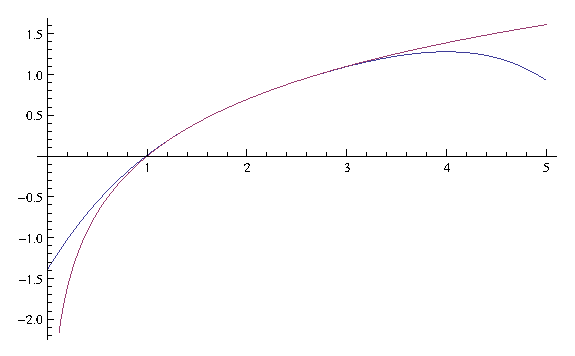
\includegraphics{continuous/series/lnxtaylor}
      \end{center}
      \caption{A plot of $\ln x$ and our Taylor approximation.}
    \end{figure}
  \end{sol}
\end{ex}
% \begin{ex}
%   Find a Taylor series of
%   \[ f(x) = \sin x \]
%   at $x=0$.
%   \begin{sol}
%     We see odd numbers appear.
%     \begin{align*}
%       \sin x &\approx \left[ \sin 0 + \cos x (x-0)^1 + \frac{-\sin x (x-0)^2}{2!} -
%       \cos x (x-0)^{3}{3!} + \frac{\sin x (x-0)^4}{4!} \right]_{x=0} + \frac{\cos x
%       (x-0)^5}{5!}
%       \cdots
%       \\
%       \sin x &\approx 0+x - \frac{x^3}{3!} + \frac{x^5}{5!} + \cdots
%   \end{align*}
%   We could, in other words, write this as
%   \[ \sin x = \sum_{n=0}^\infty \frac{(-1)^n \cdot x^{2n+1}}{(2n+1)!} \]
%   This is a \emph{power series about} $x=0$.
%   Since we have a power series, we can find its \emph{interval of convergence.}
%
%   \[ \lim_{n\to\infty} \frac{(-1)^{n+1} x^{2(n+1)+1}}{[2(n+1)+1]!} \]
%   An $x^2$ factors.
%  We're left with   \[ \lim_{n\to\infty} \frac{(-1)^{n+1}
%    x^{2(n+1)+1}}{[2(n+1)+1][2(n+1]} \]
%   The interval of convergence is $-\infty<x<\infty$.
%   \end{sol}
% \end{ex}
